\documentclass[preprint]{elsarticle}
\usepackage{lineno,hyperref}
\usepackage[citestyle=plain]{biblatex}
\modulolinenumbers[5]
\journal{Planetary and Space Science}
\begin{document}

\begin{frontmatter}

\title{Geological Moon/Mars analog simulation in volcanic region of the Eifel, Germany}

\author[esa,uw,wsosp]{Harasymczuk M.}
\author[esa,ilewg,vu]{Vos H. C.}
\author[esa]{Kołodziejczyk A.}
\author[esa]{Kraiński M.}
\author[charles,qed]{Davidová L.}
\author[esa]{Mirino M.}
\author[esa,ilewg,vu]{Foing B. H.}
\author[esa,ilewg]{Eifel ILEWG Euro MoonMars 2016 & 2017 support team}

\address[esa]{ESA ESTEC, Postbus 299, 2200 AG Noordwijk, NL}
\address[ilewg]{International Lunar Exploration Working Group}
\address[vu]{Vrije Universiteit Amsterdam}
\address[charles]{Charles University}
\address[qed]{QED Group}
\address[uw]{University of Warsaw}
\address[wsosp]{Polish Air Force University}

\begin{abstract}
During the EVA simulations performed in Eifel, Germany region the set of European Space Agency scientists and research collaborators have tested the human-robotic partnership, EVA procedures and schedule for geological sampling of the sedimentary layers in former volcanic activity location. This activities are strictly correlated with the Moon Village concept introduced by European Space Agency.
\end{abstract}

\begin{keyword}
Keywoards: Geology\sep Analog\sep Moon\sep Mars\sep Extravehicular Activity\sep EVA
\end{keyword}

\end{frontmatter}
\linenumbers

\section{Introduction}
Analog simulations have a crucial role in preparing space agencies for exploration of other celestial bodies. The main objective is to test procedures, tools and equipment for future use in those cutting-edge projects. As the Extravehicular Activity (EVA) is the most crucial part of the mission, we need to put a lot of effort on communication, timelines, checklists and astronaut training itself.

During the EVA simulations performed in the Eifel, Germany region, a set of European Space Agency scientists and research collaborators have tested human-robotic partnership, EVA procedures and schedules for geological sampling of the sedimentary layers in a former volcanic activity location. This activities are strictly correlated with the Moon Village concept introduced by Johann-Dietrich Woerner, European Space Agency Director General and Bernard Foing, ILEWG Executive director and ESA Chief Scientist & Senior Exploration Officer \cite{ref18}\cite{ref19}.

\section{Context}

\subsection{The Eifel and Moon geology}
The simulation took place in the Eifel volcanic region in the vicinity of Mendig, Germany. The place has been chosen because of past volcanic activity and rich and yet easy to access sedimentary layers. The Eifel is located in the West of Germany and is part of the Variscan Mountain belt. The Eifel was an active volcanic area during the Tertiary and Quaternary. This volcanic activity is believed to be the result of hot mantle material rising which resulted in the Eifel hotspot \cite{ref13}. This volcanism shaped the landscape of the Eifel by the formation of volcanic craters, volcanic tuff and lava streams. Even though it is believed to be still active, the largest eruption occurred approximately 12.900 years ago, when an eruption resulted in the Laacher See volcanic site \cite{ref14}. This eruption produced big amounts of pyroclastic deposits near the eruption site, but also in thin ash layers that can be found in sediments throughout Europe. This explosion formed a crater which is now a lake called the Laacher See. The locations of EVAs were near the Laacher See, next to the Wingertsbergwand, a well-known outcrop. This area consists of thin layers of volcanic ash and pumice that were formed during the aforementioned Laacher See eruption.

This site and the area of the Eifel were, besides several logistic factors, chosen because of some geological similarities with the Moon. The Moon is known for having volcanic deposits on its surface and pyroclastic materials have been found in lunar samples \cite{ref15}. An example of pyroclastic areas on the Moon is the Taurus-Littrow region, which is the landing site for the Apollo 17. During the Apollo 17 mission pyroclastic rocks were sampled for dating because it was assumed that the pyroclastic material from that region could be relatively young and can therefore represent the presence of volcanic vents. Even though the pyroclastic deposits were relatively old, 3.5 Ga, there is still an interest in pyroclastic rocks on the Moon because they hold information on the volcanic history of the Moon. Remote sensing data from a high-spatial-resolution UV/VIS camera from the Moon has been obtained during the Clementine mission and can be used for analysis of the surface of the Moon \cite{ref16}.

Similar analysis can be performed on the pumice during EVA missions using a remotely controlled spectrometer. Simulation crew has identified two distinct locations that were representative examples to test human-robotic interactions together with geologic EVA procedures. Both locations consisted of outcrops with pyroclastic deposits from the Laacher See eruption. Professionally trained geologist had chosen suitable place to conduct the analog mission before the rest of the crew arrived at the location of the simulation.

\section{Campaign description}
During the simulation, the crew has prepared three distinct Extravehicular Activities. Each one of them had different objectives. To demonstrate in situ resource utilisation possibilities, the crew has performed research on growing cress on Eifel regolith simulant samples. It was conducted in ESTEC Life Sciences laboratory after field studies.

\subsection{Materials and methods}

\subsubsection{The spectrometer}
The USB4000 (Ocean Optics) is a relatively small spectrometer that measures in the UV/VIS spectrum. The size makes the spectrometer mobile and suitable to use in the field and on a lander or a rover. However, there are clear restrictions in using this spectrometer for analyses, the first restriction being the fact that a UV/VIS spectrum gives very restricted information about measured surface compared to an infrared spectrum and the relatively high amount of noise and systematic effects makes this spectrometer less suitable for precise measurements. The spectrometer was installed on the ILEWG ExoGeoLab lander and controlled remotely, see Figure 1. During the field campaign, sunlight was used as light source for the spectroscopy measurements. However, a high integration time of 4 to 6 seconds was necessary to reach a usable light intensity. Because of the high integration time a measurement, 5 scans to average were applied instead of 10 to 20 scans to average \cite{ref8}. The high integration time could have made the analyses more sensitive to changes, such as weather changes. A dark spectrum was measured before the EVA, which means that the dark spectrum could have changed slightly when the analyses were done. The reference spectrum was measured using a white surface on which the sample can be placed for sample analyses. SpectraSuite has been used as the interface between the spectrometer and the computer.

\begin{figure}
\centering
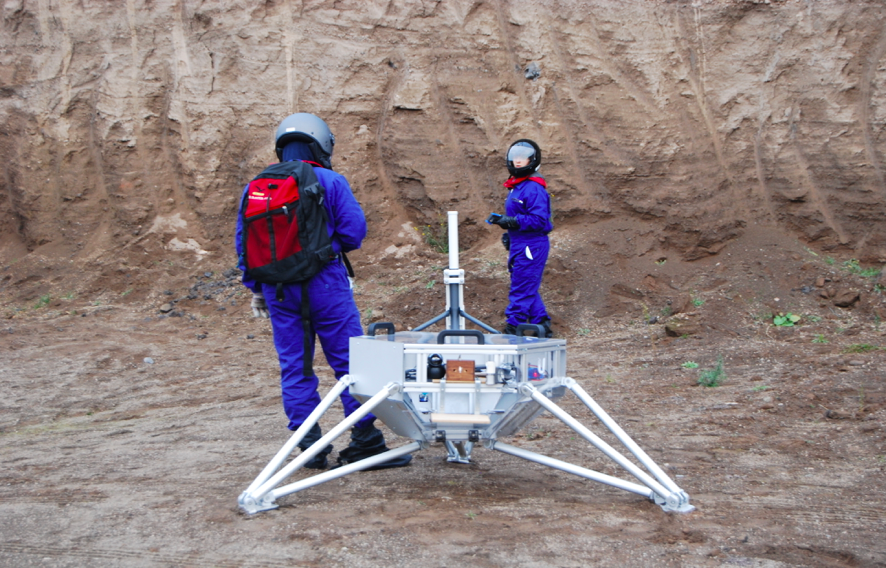
\includegraphics{img/figure01.png}
\caption{ILEWG ExoGeoLab lander with remotely controlled USB4000 spectrometer and rover.}
%\label{fig:f01}
\end{figure}

\subsection{Extravehicular Activities}

\subsubsection{The first EVA}
During the first EVA the main objective was to set-up a remote controlled telescope, which was later used to identify interesting and noteworthy objects. Before the first simulation, the analog astronaut crew started to prepare for the EVA. In the meantime, the engineering crew prepared the lander and remote controlled rover for deployment and simulated descent and landing on the ground. During the first EVA crew members' tasks were to:
\begin{itemize}
\item identify and take the contingency sample,
\item establish and test the radio communication with simple and complex commands,
\item map the vicinity of lander for possible radio communication problems,
\item photograph the location of the rover and nearby rock wall,
\item secure the lander,
\item check wireless connection of the computer systems between lander and habitat,
\item setup and calibrate the spectrometer analysis device,
\item photograph the soil and rock sampling location,
\item identify and sample the most interesting elements of the sedimentary layer,
\item photograph the rock to outcrop,
\item outcrop rock samples and collect in plastic bags, photograph and mark the bags,
\item test rover mobility near the landing site
\item deliver the rock samples using the rover to the spectrometry analysis device on lander,
\item conduct spectrometry analysis from the habitat using remote control.
\end{itemize}

\begin{figure}
\centering
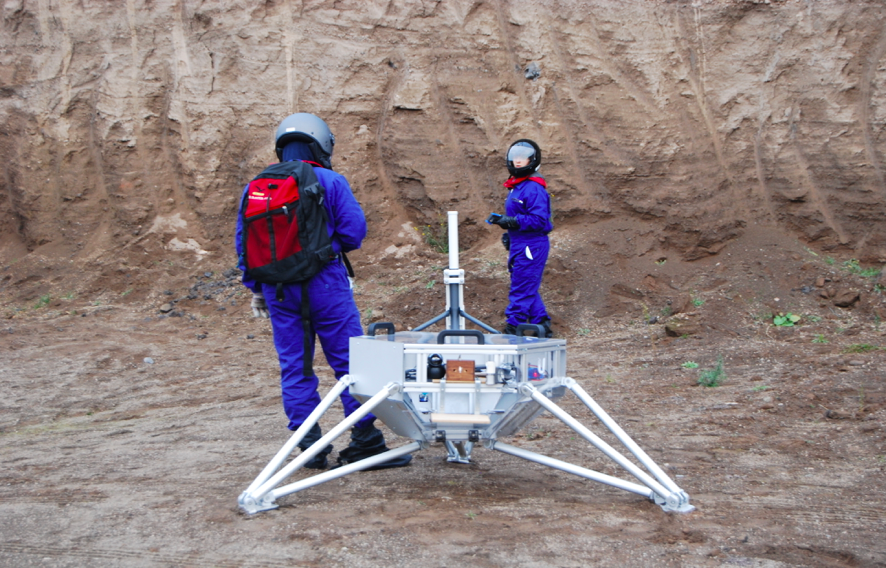
\includegraphics{img/figure02.png}
\caption{Two astronauts and the ILEWG ExoGeoLab lander during an analogue Moon EVA.}
%\label{fig:f02}
\end{figure}

\subsubsection{The second EVA}
The second EVA's main objective was to secure lander's access to power using solar panels and to do geological field work. Moreover the team had to:
\begin{itemize}
\item investigate more in-depth details of the sedimentary layers,
\item photograph with high resolution camera the field of work,
\item outcrop and collect rock samples to marked bags,
\item identify more detailed location for future EVAs,
\item test the suit for ease of movements,
\item test psychological aspects of the EVA,
\item test an emergency procedure for EVA termination because of solar flare coming and loss of communication.
\end{itemize}

\subsubsection{The third EVA}
The third EVA's main objective was to test rover capability to perform tasks in extremely rough terrain and for the astronaut Biologist to take a ground sample to identify signs of life. This EVA has been performed in dim light conditions with limited visibility. Tasks for the EVA crew were to:
\begin{itemize}
\item test the rover movement capabilities in rough terrain,
\item identify and collect biological samples for further analysis,
\item test the rover lights,
\item test rover's capability to assist astronauts with light,
\item test in-the-field rover control using portable antenna and sidearm joystick,
\item test radio communication procedures.
\end{itemize}

\subsection{Plant Growth on Eifel Regolith Simulant}
In order to analyze growth rate in plants on regolith soil, 10 seeds of cress Lepidium sativum (Superseeds, NL) per pot were planted in 4 copies of subsequent soil types: 20 g of autoclaved (2h in 120°C) Eifel regolith simulant soil (RA), 20 g of autoclaved Eifel regolith simulant soil with 2 ml of nutrients (KNOP medium \cite{ref17}), (RAN), 20 g not autoclaved Eifel regolith simulant soil (R), 10g of peat (S), 10 g of autoclaved peat (SA). Lowered mass of peat (Potgrond universel, BVB Gardening, NL), was used to obtain the same volume of soil in experimental pots. 35 transparent pots were used in the experiment. 20 pots containing seeds, 4 pots per one soil type, and 15 blank pots only with various types of used soils to control contamination processes, 3 pots per one soil type (Figure 3).

\begin{figure}
\centering
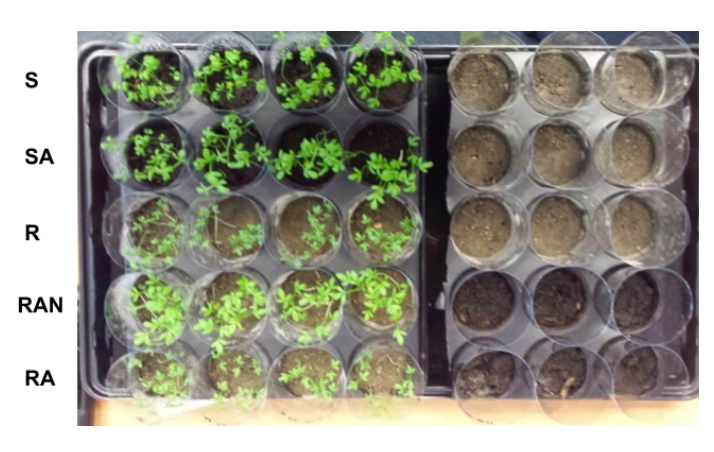
\includegraphics{img/figure03.png}
\caption{Experimental setup for plant growth analysis on regolith simulant Eifel soil. Left side with rows of cress: RA - autoclaved regolith, RAN - autoclaved regolith with nutrients, R - regolith, SA - autoclaved peat, S - peat. On the right side soil samples without plants to analyze contamination effects during watering and cultivation period. Regolith soil differs in color comparing to the dark peat.}
%\label{fig:f03}
\end{figure}

Two week long experiment was performed in a microharvester (MicroHarvester V3, Germany), in 32°C with 12:12 L:D light/dark conditions (12 hours lights on, 12 hours darkness). Every second day plants were watered with 5 ml of distilled water. Growth rate analysis was performed based on data collected in four subsequent days of the fastest morphological plant transformation (5th, 6th, 7th and 8th day of the experiment), by using imaging method. Images were processed and measured in ImageJ Software. Obtained data was analyzed in Excel.

\subsection{Psychosocial investigation}
Three EVAs were conducted always by two analogue astronauts with support from mission control centre. Each EVA was performed by different analogue astronauts of various professions (geologist, biologist, engineer, psychologist etc.) and research focus as mentioned in section 3.2 Extravehicular Activities. Psychosocial aspects of the simulation were investigated.

Research indicates that the relationship between astronaut crew and mission control may be problematic \cite{ref21}\cite{ref22}. From this reason this psychosocial investigation included both - the astronauts as well as the mission control personnel - mainly Capsule Communicator (CapCom). Several methods were applied. Observation was conducted during the EVAs and interviews with all analogue astronauts and Capsule Communicators were performed in the post-simulation phase. The main intention of the psychosocial research was to study communication.

Sociomapping method \cite{ref20}\cite{ref23} was used to visualize the interactions between analogue astronauts and CapCom. Sociomapping is an psychodiagnostic method that enables visualisation of relations within a team. The height of the sociomap reflects the intensity of a certain aspect (in this case the quality communication). Colours vary from red (the highest intensity) through yellow and green to dark blue (lowest intensity). The position of individual elements (people) stands for the position in the team and indicates the psychological proximity among crewmembers \cite{ref20}\cite{ref23}. Sociomaps were created by Socimapping software \cite{ref20} and were based on the data collected as a part of the interviews by using closed five point scale.

\section{Results}
During the second EVA the crew performed a basic geological analysis of the volcanic outcrop. The studied area was selected based on the good variability and visibility of the layers with the objective to collect samples with different characteristics. In this way it was possible to obtain deeper information of all the outcrop with a secondary study performed in laboratory.

The outcrop showed eruptive sequence formed by layers with sub-horizontal stratigraphy composed by cinder deposits alternate to cross laminations in some phyroclastic deposits, formed by pumice stone with one to ten millimetre dimensions, where it was possible also observe some accessory block (Figure 4). The characteristic mentioned above suggest a past turbulent phyroclastic flux. The second crew of astronauts selected samples from each layer using indication from the mission control station. In the paragraph the results obtained after the spectroscopy analyses are presented.

\begin{figure}
\centering
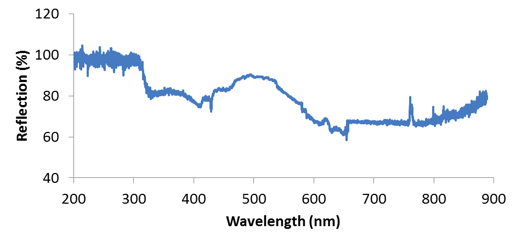
\includegraphics{img/figure04.png}
\caption{In this figure we show the layers that we used to collect the samples. In the image on the left it is possible to observe a detail of the outcrop where phyroclastic and cinder deposits are alternated. In the image on the right it is present one accessory block.}
%\label{fig:f04}
\end{figure}

\subsection{Field spectroscopy, imaging and sampling}
Several spectroscopy measurements in the UV/VIS spectrum were performed using a remotely controlled USB4000 spectrometer, during a field campaign in the Eifel volcanic area in Germany. The data that was obtained during the field measurements was compared to the data obtained from laboratory analyses to determine the reliability of field spectroscopy analyses. By determining the errors that can occur during field measurements we hope to establish better conditions for field spectroscopy and an improved calibration method to minimize errors for future field measurements.

\subsubsection{In-situ results}
Figure 5 shows the reference spectrum from the sample analysis and Figure 6 shows the spectrum of one of the volcanic rocks that was sampled during the field campaign. Figure 6 shows a number of anomalies that are likely not caused by absorption bands from the sample. A high reflection value around 760 nm and relatively more absorption around 430 nm and 590 nm are examples of such anomalies.

\begin{figure}
\centering
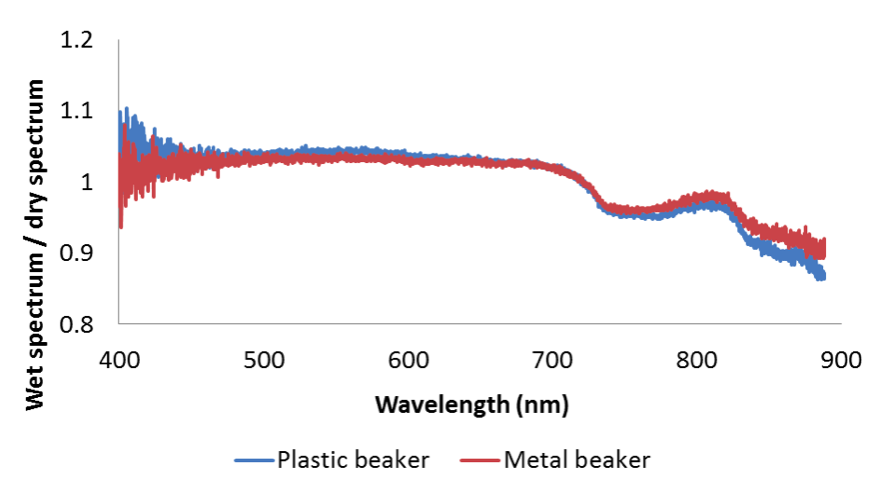
\includegraphics{img/figure05.png}
\caption{The reference spectrum that was used to analyse the sample during the field campaign.}
%\label{fig:f05}
\end{figure}

\begin{figure}
\centering
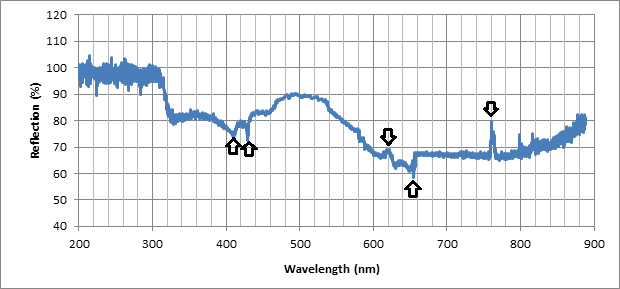
\includegraphics{img/figure06.png}
\caption{The reflection of a volcanic sample from the Eifel volcanic area measured during a Moon EVA.}
%\label{fig:f06}
\end{figure}

\subsubsection{Post campaign measurements}
As stated before, sample measurements were conducted again in laboratory conditions, after the campaign. The analyses were performed using the the same spectrometer (USB4000), in a dark environment with incandescence light source. This light source does not emit UV light and it makes spectrum analysis below 400 nm impossible. Figure 7 shows the reflection spectrum of the volcanic sample from the laboratory measurement and from the field measurement. The integration time for the laboratory measurements was 200 milliseconds and the final result was generally an average of 20 measurements. A dark spectrum was measured before each sequence and the reference spectrum was determined before each measurement.

\begin{figure}
\centering
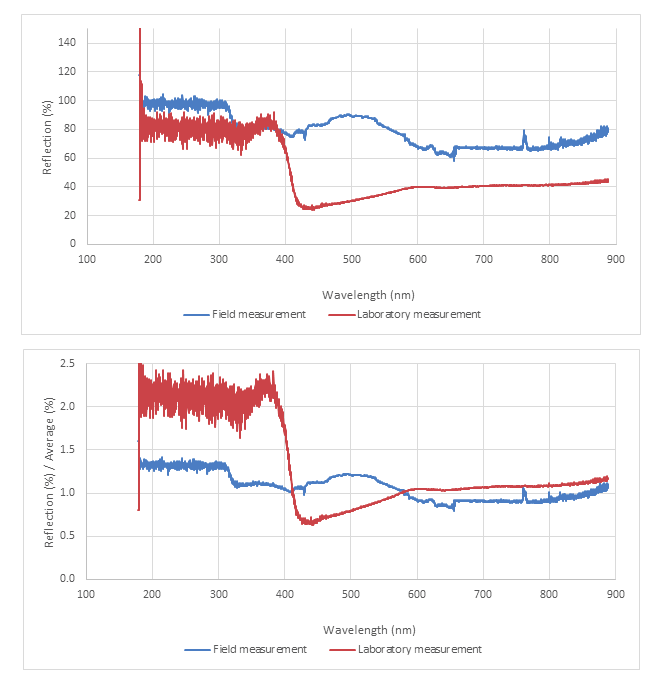
\includegraphics{img/figure07.png}
\caption{The spectra of the volcanic rock that was sampled during the EVA and measured with both field and laboratory analyses.}
%\label{fig:f07}
\end{figure}

When comparing the results from the field measurements it is visible that the spectras differ from from each other. These differences can be caused by changes in weather conditions or errors in the reference spectrum. To determine the possible influence of the weather conditions on the reference spectrum the spectrum of a sky during different weather conditions were analysed. Figure 8 shows the spectra of the reference spectrum from the field analyses and from a clouded and a clear sky, which was analysed with an integration time of 300 ms, the spectrum of direct sunlight which was measured with an integration time of 3.8 ms and. There are clear differences visible between these spectra. For example, the spectrum of the clear sky shows a high intensity in the blue spectrum, which can be expected. However, all the spectra show absorption bands that represent the Fraunhofer lines. These lines are caused by absorption by for example oxygen (686 nm, 759 nm and 823 nm nm), helium (588 nm) and hydrogen (410 nm, 434 nm, 486 nm and 656 nm, also known as the Balmer lines)

Figure 9 shows the values from Figure 8 divided by the reference spectrum from the EVA. By analyzing the difference between these spectra and comparing it to the sample analyses it is possible to determine the influence the weather conditions could have had on the sample analyses during the EVA. A peak at 759 nm is visible in all the ratios and can therefore probably be caused by weather conditions since it is caused by the absorption by oxygen. Between 400 nm and 500 nm the measurement during the EVA shows a high reflectance compared to the laboratory analyses. This can partially be caused by less direct sunlight. However, if a change of weather would have caused a disturbance in the spectrum during EVA, a question that remains is why certain anomalies, such as an increase at 686 nm, are not visible.

\begin{figure}
\centering
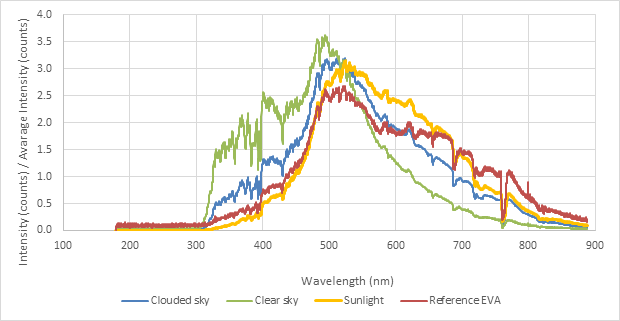
\includegraphics{img/figure08.png}
\caption{The spectrum of different natural light sources and the reference spectrum that was measured and used during the EVA.}
%\label{fig:f08}
\end{figure}

\begin{figure}
\centering
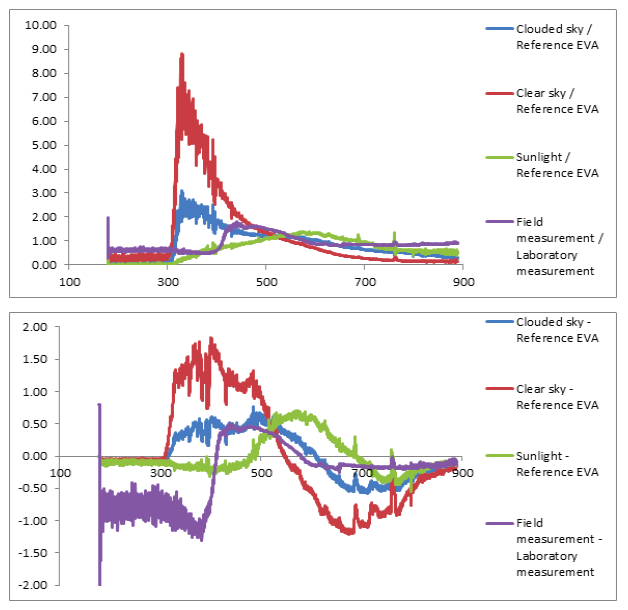
\includegraphics{img/figure09.png}
\caption{The spectrum of different weather conditions compared to the spectrum that was measured during the EVA and used as a reference spectrum.}
%\label{fig:f09}
\end{figure}

We hope to improve the conditions for the measurements and create a calibration method by being aware of the errors that can occur during field spectroscopy analyses. Spectroscopy analyses in the UV/VIS spectrum is limited in its practical use. However, being aware of the problems that arise during field spectroscopy in UV/VIS spectrum can also be taken into account during measurements in NIR and IR spectra. The measurements will be repeated during a planned field experiment in February 2017 to determine the changes in the spectrum by changing parameters. By adding an extra light source near the spectrometer we expect to improve the results from the spectroscopy analyses. This will also make it possible to measure using a smaller integration time and a higher scans to average to improve the result. Finally we will look at the difference in using a white surface or the sky as reference spectrum.

\subsection{Human/robotic partnership and rover operations results}
During the EVAs, astronauts were supported by a mobile rover (shown on Figure 1), built by the crew engineer from of-the-shelf components. It is operated remotely with a joystick, via a WiFi network, from the habitat (with visual feedback from an on board camera) or by one of the astronauts (without the feedback). For two of three missions, the rover was operated from the habitat. During the last mission, one of the astronauts operated the rover from an arm mounted control panel. Both ways have proved to be effective and efficient.

Before operations, it served as a survey device, which was deployed before the EVA in order to find best sampling areas. During an EVA, the rover was used as a sample storage and transport device, from the sampling area to the lander or habitat, so astronauts could focus on collecting samples, mobility and communication with MCC.

From the construction view, the rover is based on a 6WD Wild Thumper \cite{ref27} all-terrain chassis, powered by a 5000 mAh Redox 2S LiPo battery. Motors are driven by 2 Pololu 18v25 Motor Drivers \cite{ref26}. The main computer, Raspberry Pi 3 model B \cite{ref25}, runs Raspbian with Robot Operating System framework \cite{ref24} for motor and camera control, and WiFi communication with the operator. Such configuration allows engineers working on the system for a lot of flexibility and provides many development areas. The development of the rover was supported by National Geographic.

Currently, a robotic arm is in development. It will allow the rover to pick up samples and perform other tasks requiring manipulation. There are works aiming to integrate additional sensing tools with with the rover such as a GPS sensor for marking sampling areas, implementing visual based 3D mapping technologies for creating a full 3D map of the environment, magnetometer for measuring magnetic field anomalies in the area, spectrometer for making in-situ measurements or even Geiger counter for radiation level measurements. Also work is made to improve the storage capabilities of the rover, so that it can also transport various tools and meters for the astronauts. Additional work might be done to assemble a deployable meteorological station to measure temperature, pressure, humidity dust and wind.

\subsection{Morphological changes and diverse plant growth on the regolith simulant soils}
Plant development depends on environmental factors such light, humidity and temperature, seed quality, contaminations and soil type. In laboratory conditions we could control all parameters, so observed differences were only the effect of soil type and added nutrients. In the 4th day of the experiment plants already emerged from seeds in subsequent values: 60% of plants in RA, 85% in RAN, 95% in R, 90% in SA, and 67% in S. This results suggest that emerging cress from seeds was not affected by the quality of soil, however influence of nutrients could be seen. On the next 4 following days the lengths of stems were measured and visualized in Figure 7.

\begin{figure}
\centering
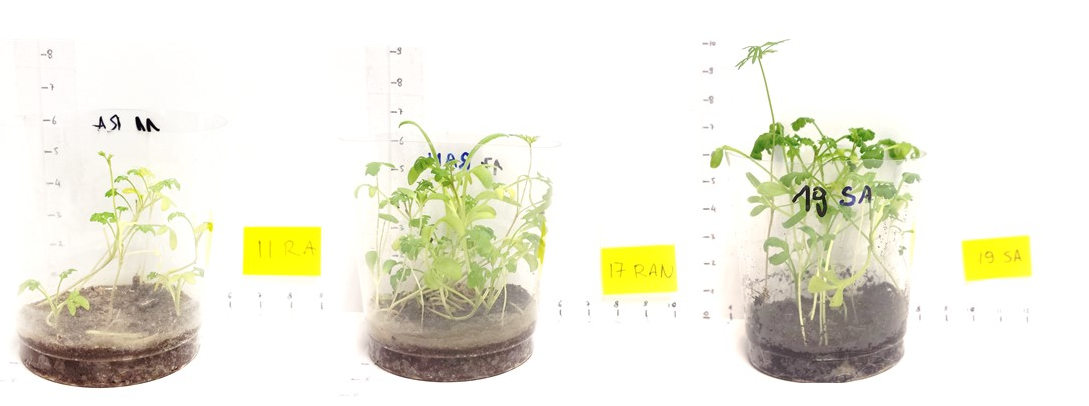
\includegraphics{img/figure10.png}
\caption{Imaging method used in the plant growth analysis. For each testing sample lengths of plant stems were measured and standardized to the imaged scale. Significant morphological changes were observed between compared soil types. This images visualize 12 days old cress.}
%\label{fig:f10}
\end{figure}

\begin{figure}
\centering
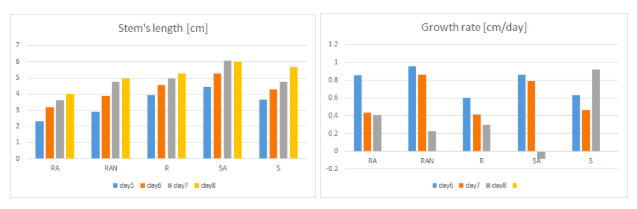
\includegraphics{img/figure11.png}
\caption{Average stem length [cm] and average growth rate [cm/day] of cress Lepidium sativum.}
%\label{fig:f11}
\end{figure}

In general, we observed that plant development was different in different types of soil (Figure 10, 12). In particular, plants grown on the regolith simulant have had thinner leaves and were shorter than the plants grown on peak or regolith with nutrients (Figure 10, 12). Interestingly, autoclaved peak (SA) was better for the plant development than not autoclaved one (S). This suggests, that microorganisms living in not autoclaved soil suppress plant development by evoking stress responses. The growth process reached maximal value in the 6th day of the experiment on regolith soil. The highest averaged growth rate 0.96 cm/day was observed for plants growing on the nutrient-enhanced regolith simulant (RAN).

\begin{figure}
\centering
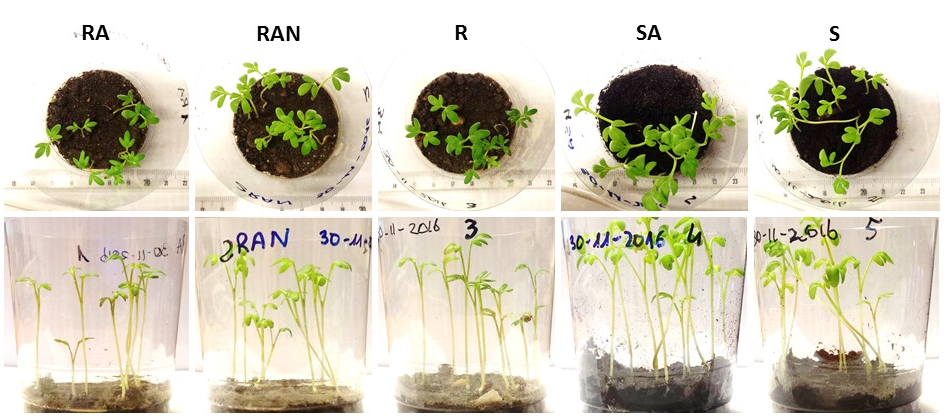
\includegraphics{img/figure12.png}
\caption{9th days old cress on different types of soil: RA - autoclaved regolith simulant, RAN - autoclaved regolith simulant with nutrients, R - regolith simulant, SA - autoclaved peak, S - peak. Visible changes in leaves and stem sizes. Characteristic T-shaped leaves in RA and R, comparing to Umbrella-shaped nourished leaves in other samples.}
%\label{fig:f12}
\end{figure}

Our studies revealed, that regolith simulant enriched with nutrients, could be used for plant cultivation in space. More studies need to be done to optimize the plant growth on regolith soil.

\subsubsection{Spectroscopy analyses}
For this experiment we will focus on the visible spectrum of green vegetation which is controlled by the presence of chlorophyll. Chlorophyll can be found in algae and plants and is necessary for photosynthesis and gives these organisms their green colour. This is the result of the fact that chlorophyll mainly absorbs light from the blue and red areas of the electromagnetic spectrum and absorbs poorly from the green spectrum, which results in the green colour of chlorophyll. There are roughly two types of chlorophyll: chlorophyll a and b. The exact absorption of chlorophyll is difficult to measure precisely since the spectrum can be influenced by the extraction method, the solvent and the spectrometer. Chlorophyll a absorbs between 428 and 432 nm and 660 and 665 nm, chlorophyll b absorbs between 452 and 469 nm and between 642 and 652 nm.

Figure 13 shows the results from spectroscopy analyses performed on the last day of the experiment (21st day cress). At the moment of the measurements, a lot of plants did already started to dry out. This is also visible in the spectra of these plants. An example is measurement R3 which shows less absorption in the blue and red area compared to the green spectrum. To determine the difference in absorption two ratios were calculated. This ratio is based on the lowest reflectance value between 460 and 540 nm (Minimum 1) and between 620 and 700 nm (Minimum 2), and the highest reflection between 530 nm and 580 nm (Maximum 1) and between 700 and 770 nm (Maximum 2). Figure 14 shows the ratio of these samples from the beginning (the 8th day) and the end (the 21 day) of the experiment. There is a clear distinction between the measurements on the beginning of the experiments and the measurements at the end of the experiment. This can be caused by drying of the plants, which results in less absorption and reflection of chlorophyll.

\begin{figure}
\centering
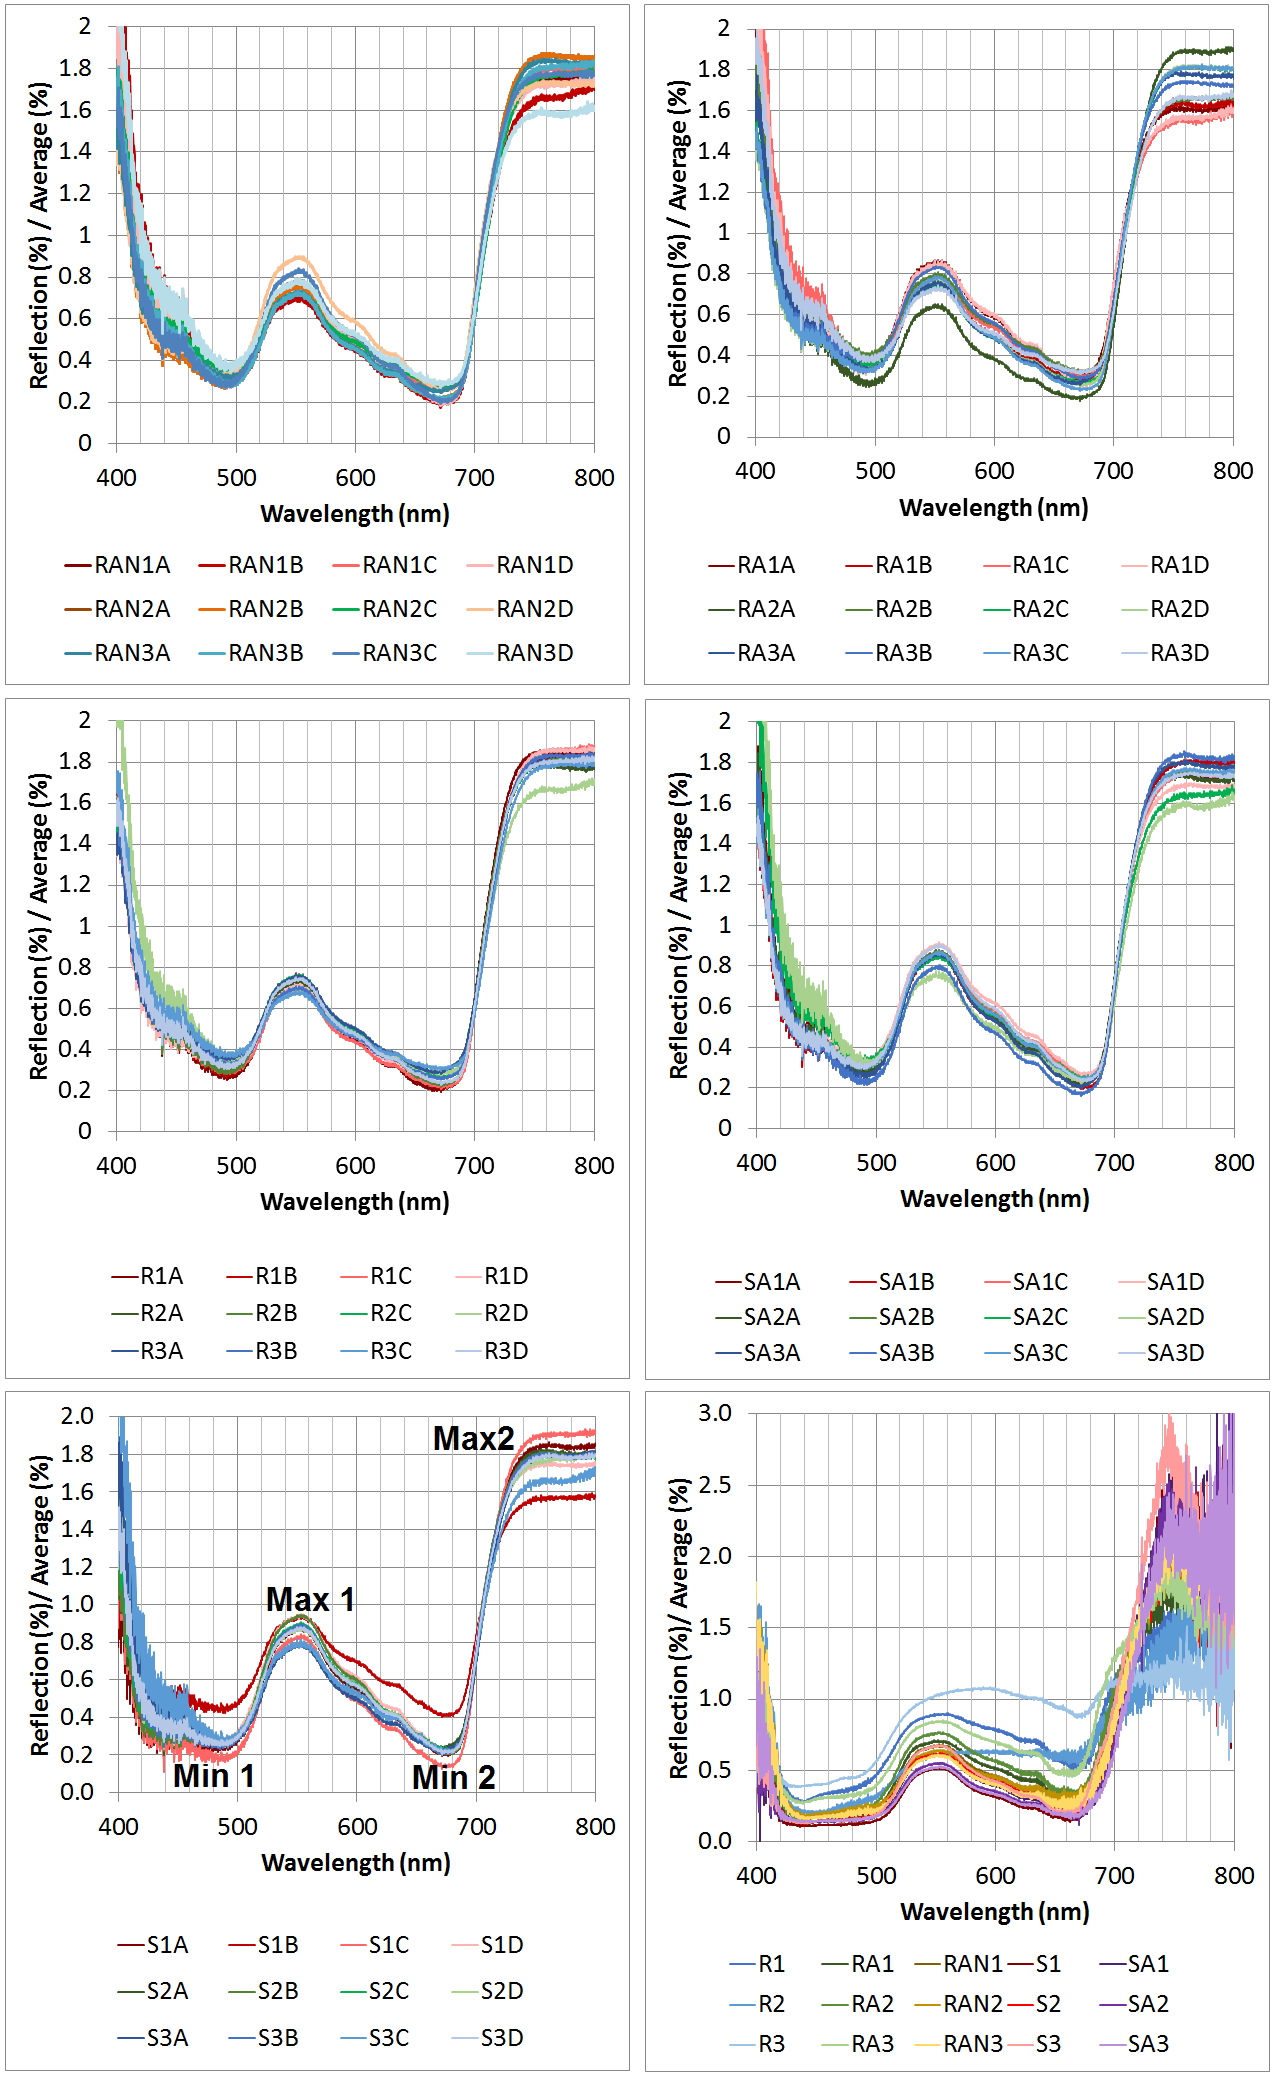
\includegraphics{img/figure13.png}
\caption{The spectrum of the leafs from the plant experiment.}
%\label{fig:f13}
\end{figure}

\begin{figure}
\centering
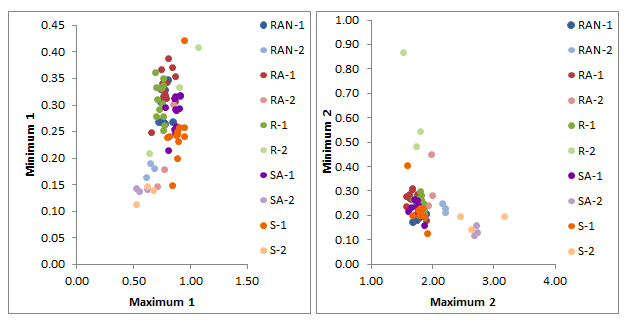
\includegraphics{img/figure14.png}
\caption{The ratios of the maximum and minimum values measured during the 8th day (...-1) and 21st day of the experiment (...-2). A clear division is visible between these two moments of analyses.}
%\label{fig:f14}
\end{figure}

\subsection{Psychosocial investigation}
Astronauts as well as mission control personnel were observed during the EVAs and interviewed in the post-simulation phase.

\subsubsection{Sociomapping}
Sociomaps were created by Sociomapping software \cite{ref20}. There are three sociomaps (Figures 15-17) presented - one from each EVA. These sociomaps visualize the quality of communication among astronauts and CapCom. The visualization was created from collected data, based on subjective evaluation of participants.

The sociomap of the first EVA (Figure 15) shows very close communicational relationship of two astronauts and very high quality of the the communication (evaluated as "always above average") between those two individuals. CapCom is distant, marked with light blue indicating rather low quality of communication which was evaluated by astronauts between "sufficient" and "should sometimes be better".

\begin{figure}
\centering
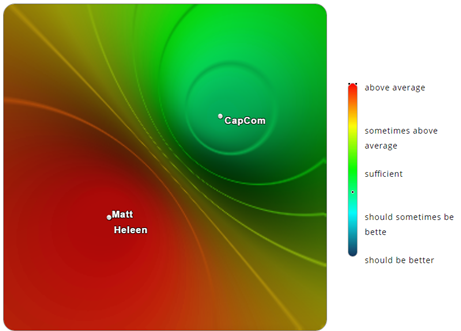
\includegraphics{img/figure15.png}
\caption{The sociomap of the quality of communication of the first EVA team.}
%\label{fig:f15}
\end{figure}

The sociomap of the second EVA also visualizes CapCom in the position that is far away from the astronauts even though the communication quality of CapCom was evaluated as sufficient. The quality of communication between astronauts and CapCom was low which could be caused by technical problems as described below.

\begin{figure}
\centering
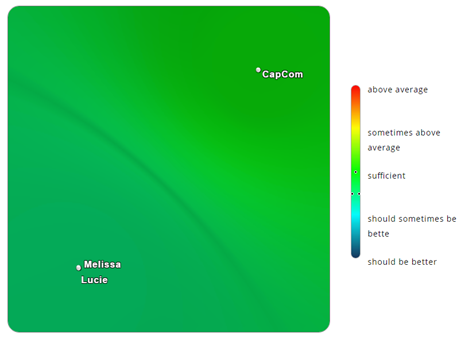
\includegraphics{img/figure16.png}
\caption{The sociomap of the quality of communication of the second EVA team.}
%\label{fig:f16}
\end{figure}

The sociomap of third EVA shows very high quality of communication. The cohesion of the team is high and includes CapCom. Overall communication quality of this EVA was above average.

\begin{figure}
\centering
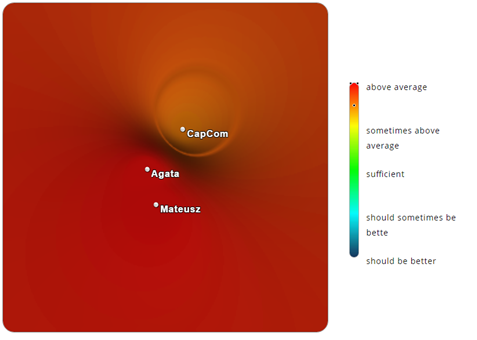
\includegraphics{img/figure17.png}
\caption{The sociomap of the quality of communication of the third EVA team.}
%\label{fig:f17}
\end{figure}

\subsubsection{Technical issues of communication}
Evaluation of technical aspects of communication was conducted as a part of the interviews. All astronauts and CapComs have evaluated on the scale from 1 (very bad) to 5 (very good, no problems) how the technical aspects of the communication during their EVA influenced the quality of communication. Figures 18-20 reflects the evaluation of two astronauts and CapCom of certain EVA.

\begin{figure}
\centering
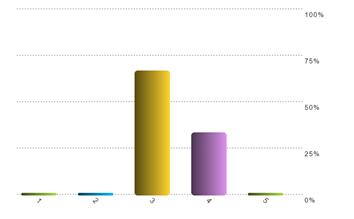
\includegraphics{img/figure18.png}
\caption{The evaluation of the technical aspects of communication of the first EVA.}
%\label{fig:f18}
\end{figure}

\begin{figure}
\centering
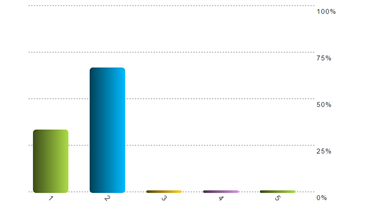
\includegraphics{img/figure19.png}
\caption{The evaluation of the technical aspects of communication of the second EVA.}
%\label{fig:f19}
\end{figure}

\begin{figure}
\centering
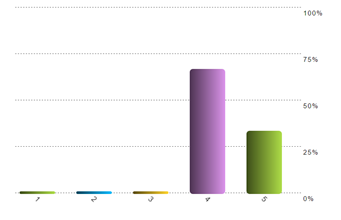
\includegraphics{img/figure20.png}
\caption{The evaluation of the technical aspects of communication of the third EVA.}
%\label{fig:f20}
\end{figure}

Results show correlation with results obtained from sociomaps (Figures 15-17). The most problematic in the scope of the technical aspects was the second EVA (Figure 19) which was also associated with the lowest communication quality among individuals (Figure 16). Due to those technical issues, the astronauts during the second EVA have missed the emergency call from mission control. The highest communication quality among participants as well as relatively positively evaluated technical aspects of communication are visible in graph of the third EVA (Figure 17, 20).

\subsubsection{Astronaut's feelings}
Analogue astronauts were individually interviewed and asked about their feelings regarding the status of analogue astronaut ("How did you feel as an astronaut?") and emotions during an EVA ("Could you describe your emotions during the EVA?"). Three out of six astronauts mentioned that they were stressed, especially in the beginning of their EVA. Three out of six astronauts mentioned high excitement connected to the being an astronaut. Other positive statements such as "fun", "nice work", "pleasant" etc. were expressed by four out of six astronauts.

Next part of the interviews has focused on perceived difficulties ("What difficulties did you have to face? And what challenges you had to overcome?"). The answers were mainly connected to the specific tasks of each individual except the difficulties caused by helmet and gloves which were mentioned by two astronauts.

Astronauts was also asked to rate their work done during EVAs on five point scale: 1 (very bad) to 5 (excellent). The ratings varied just from 2 to 4. CapComs also rated the work of the astronauts. However, their ratings were more positive and ranged from 4 to 5.

\section{Analog Extravehicular Activity operational issues}
During EVA scenarios, the team was able to identify several issues. Most of those issues were connected with communication and mission organization. The problems have been reported and elaborated upon to create a lessons learned article. Here's the list of the improvements astronauts team must introduce before the next simulation.

\subsection{Communication}
\begin{itemize}
\item train astronauts with radio communication,
\item establish common communication language,
\item introduce common linguo and alphabet,
\item pre-established radio callsigns and callouts,
\item establish protocol for emergency calls,
\item introduce radio communication culture,
\item introduce protocol for lost communication,
\item train crew to communicate intentions before activity,
\item simplify the emergency procedures,
\item investigate problems with radio communication hardware.
\end{itemize}

\subsection{Mission Organization}
\begin{itemize}
\item improve EVA scenarios,
\item make the general mission objectives more clear,
\item train more people in lander and onboard hardware assembly,
\item introduce inventory system and keep your workspace clean culture,
\item prevent chaos with spontaneously happen,
\item introduce segregated compartments with tools and spare parts,
\item log EVA events, timelines, informations,
\item keep more organized notes or use IT system support,
\item introduce briefings and debriefing.
\end{itemize}

\subsection{Extravehicular Activity}
\begin{itemize}
\item create a pre-EVA checklist: rock hammer, sample bags, size comparison marker, suit stuff, lightning,
\item create a procedure for taking pre- and post-EVA medical measurements,
\item maintain in-habitat culture while EVA is in progress,
\item shorten the pre-EVA procedure,
\item introduce a culture to work in pairs (leading EV1 and supporting EV2),
\item document in more detailed manner the field and sample before performing a tasks,
\item keep order in things and place things up in the proper places,
\item introduce on arm checklist,
\item introduce event logging for the habitat crew.
\end{itemize}

\section{Lessons learned}

\subsection{Wrap-up session}
After the simulation crew has been participating in the wrap-up session, in which the following talks were delivered:
\begin{itemize}
\item Status Moon Village activities update (B. Foing),
\item Spaceship EAC update (A. Cowley),
\item MoonMars Base Simulation (A Kolodziejczyk),
\item 1year at HiSeas Mars and MAMBA MoonMarsBase project (C. Heinicke),
\item MoonWalk (I. Schlacht/J. Rittweger/C. Inellioglu),
\item Lunar EVA simulations (M. Harasymczuk),
\item MoonMars Simulation Psychology studies (L. Davidova),
\item Material and 3D printing studies (EAC),
\item Collecting and analysing samples with robots and astronauts (M. Mirino),
\item MoonMars analogue sample spectro demo (H. Vos),
\item Virtual reality Model study of lunar polar illumination (A. Casini),
\item Sending robots to space (M. Krainski),
\item Virtual Reality Simulation Game at MoonVillage (E. Tomozei),
\item presentation by Spaceship EAC students,
\item report from ESTEC workshop & Eifel field study.
\end{itemize}

\section{Acknowledgements}
We thank participants and collaborators for the ILEWG EuroMoonMars Dec 2016 campaign at the Eifel and National Geographic for support in building the rover.

\section{Bibliography}
\bibliographystyle{plain}
\bibliography{bibliography}

\end{document}
